\section{Fitting Procedures and Errors}\label{appFitting}

\textbf{
    In this section we give more details on how we compute the VSFs and their scaling parameters.
    As described in Sect.~\ref{methods:vsf} our previous discussions are based on VSFs that are computed from average relative velocities. 
    This means the following:
}

\textbf{ 
    We map the 3D FLASH data of the original simulations \citepalias{IbanezMejia2016} onto data cubes. 
    Those cubes consists of 400$^3$ subcubes, each representing a volume of (0.1~pc)$^3$, with the centre of the cubes being close to the centres of the molecular clouds. 
}

\textbf{
    As a consequence, we can only offer a discrete representation of the velocity information. 
    No matter whether a density threshold is applied or not, this binning still represents an amount of data that is computationally hard to process.
    For deriving and analysing the VSFs we coarsen the grid of projected lag distances, $\ell_i = |\vec{\ell}|_i$, so that separates the range between 0.1 and 30~pc into only 40 equidistant bins.
}

\textbf{
    Going back to the simulated data we apply two approaches: 
    The first strategy considers the density threshold, n$_\mathrm{cloud}$.
    This means that we pick only those cells from the data cubes that contain number densities equal to or larger than n$_\mathrm{cloud}$.
    These cells represent the starting points $\vec{x}$ (see Eqs.~\rc{!!! ref !!!}).
    Our routine goes to each of these cells and calculated the lag distance to every other cell in the sample, as well as the relative velocities of the gas that is simulated within the given cells. 
    The individual lag distances are summarised into spherical shells around the starting points that range from inner radii $\ell_{i}$ to outer radii $\ell_{i+1}$. 
    By doing so, we compute the discrete VSFs presented in the main part of this paper with the relative velocities and product of denisties, $\rho(\vec{x}) \cdot \rho(\vec{x}+\vec{\ell})$, measured from cells within the individual shells.
    The code for the routine is offered in our online repository following: \rc{!!! link !!!}.
}

\textbf{
    The second approach targets the case when we do not apply any density threshold, or setting n$_\mathrm{cloud}$~=~0.
    In this case, we use python's random number generator \rc{!!! name of package !!!} to generate a set of cells within the entire data cubes that reflect 5\% of the total volume. 
    Thereby, we check that there are no duplicates within the sample.
    The so generated set of starting point is used for the analysis.
    As it is too computationally expensive to derive all relative velocities between all cells with the discrete shells, as we have done in the first approach, we derived a discrete distribution of relative velocities as function of lag distance using the Fast-Fourier-Transformation (FFT,\rc{!!! name of package !!!}) offered by python.
    These distributions are based on the same grid of lag distances we have already utilised for the spherical shells above.
    Therefore, we can use the results of the FFT in the same way as the results from the first approach to derive the VSFs.
    The code for the routine is also offered in our online repository following: \rc{!!! link !!!}.
}

\textbf{
    With both approaches we obtain a set of discrete descriptions of VSFs as function of time (as the routines have been applied for all snapshots) and lag distance (which is identical with the grid of lag distances we have introduced above).
    In order to derive the scaling parameters, $\zeta$, of the VSFs as function of time and order, we use python's \texttt{curve_fit} package to fit the power-law relation presented in Eq.~\rc{!!! ref !!!} to the measured VSFs.
    Due to the rather irregular behaviour of our VSFs at larger scales, we define the weighting function in such a way that is emphasis the region of $\ell\,\leq$~8~pc and ceases with 1~pc/$\ell$[pc]. 
    \rc{!!! check !!!}
    The similarity parameters, $Z$, are computed by applying Eq.~~\rc{!!! ref !!!} on the results of the fitting procedure, and all results are presented in Sect.~\ref{results}.
}

\begin{figure*}
    \centering
    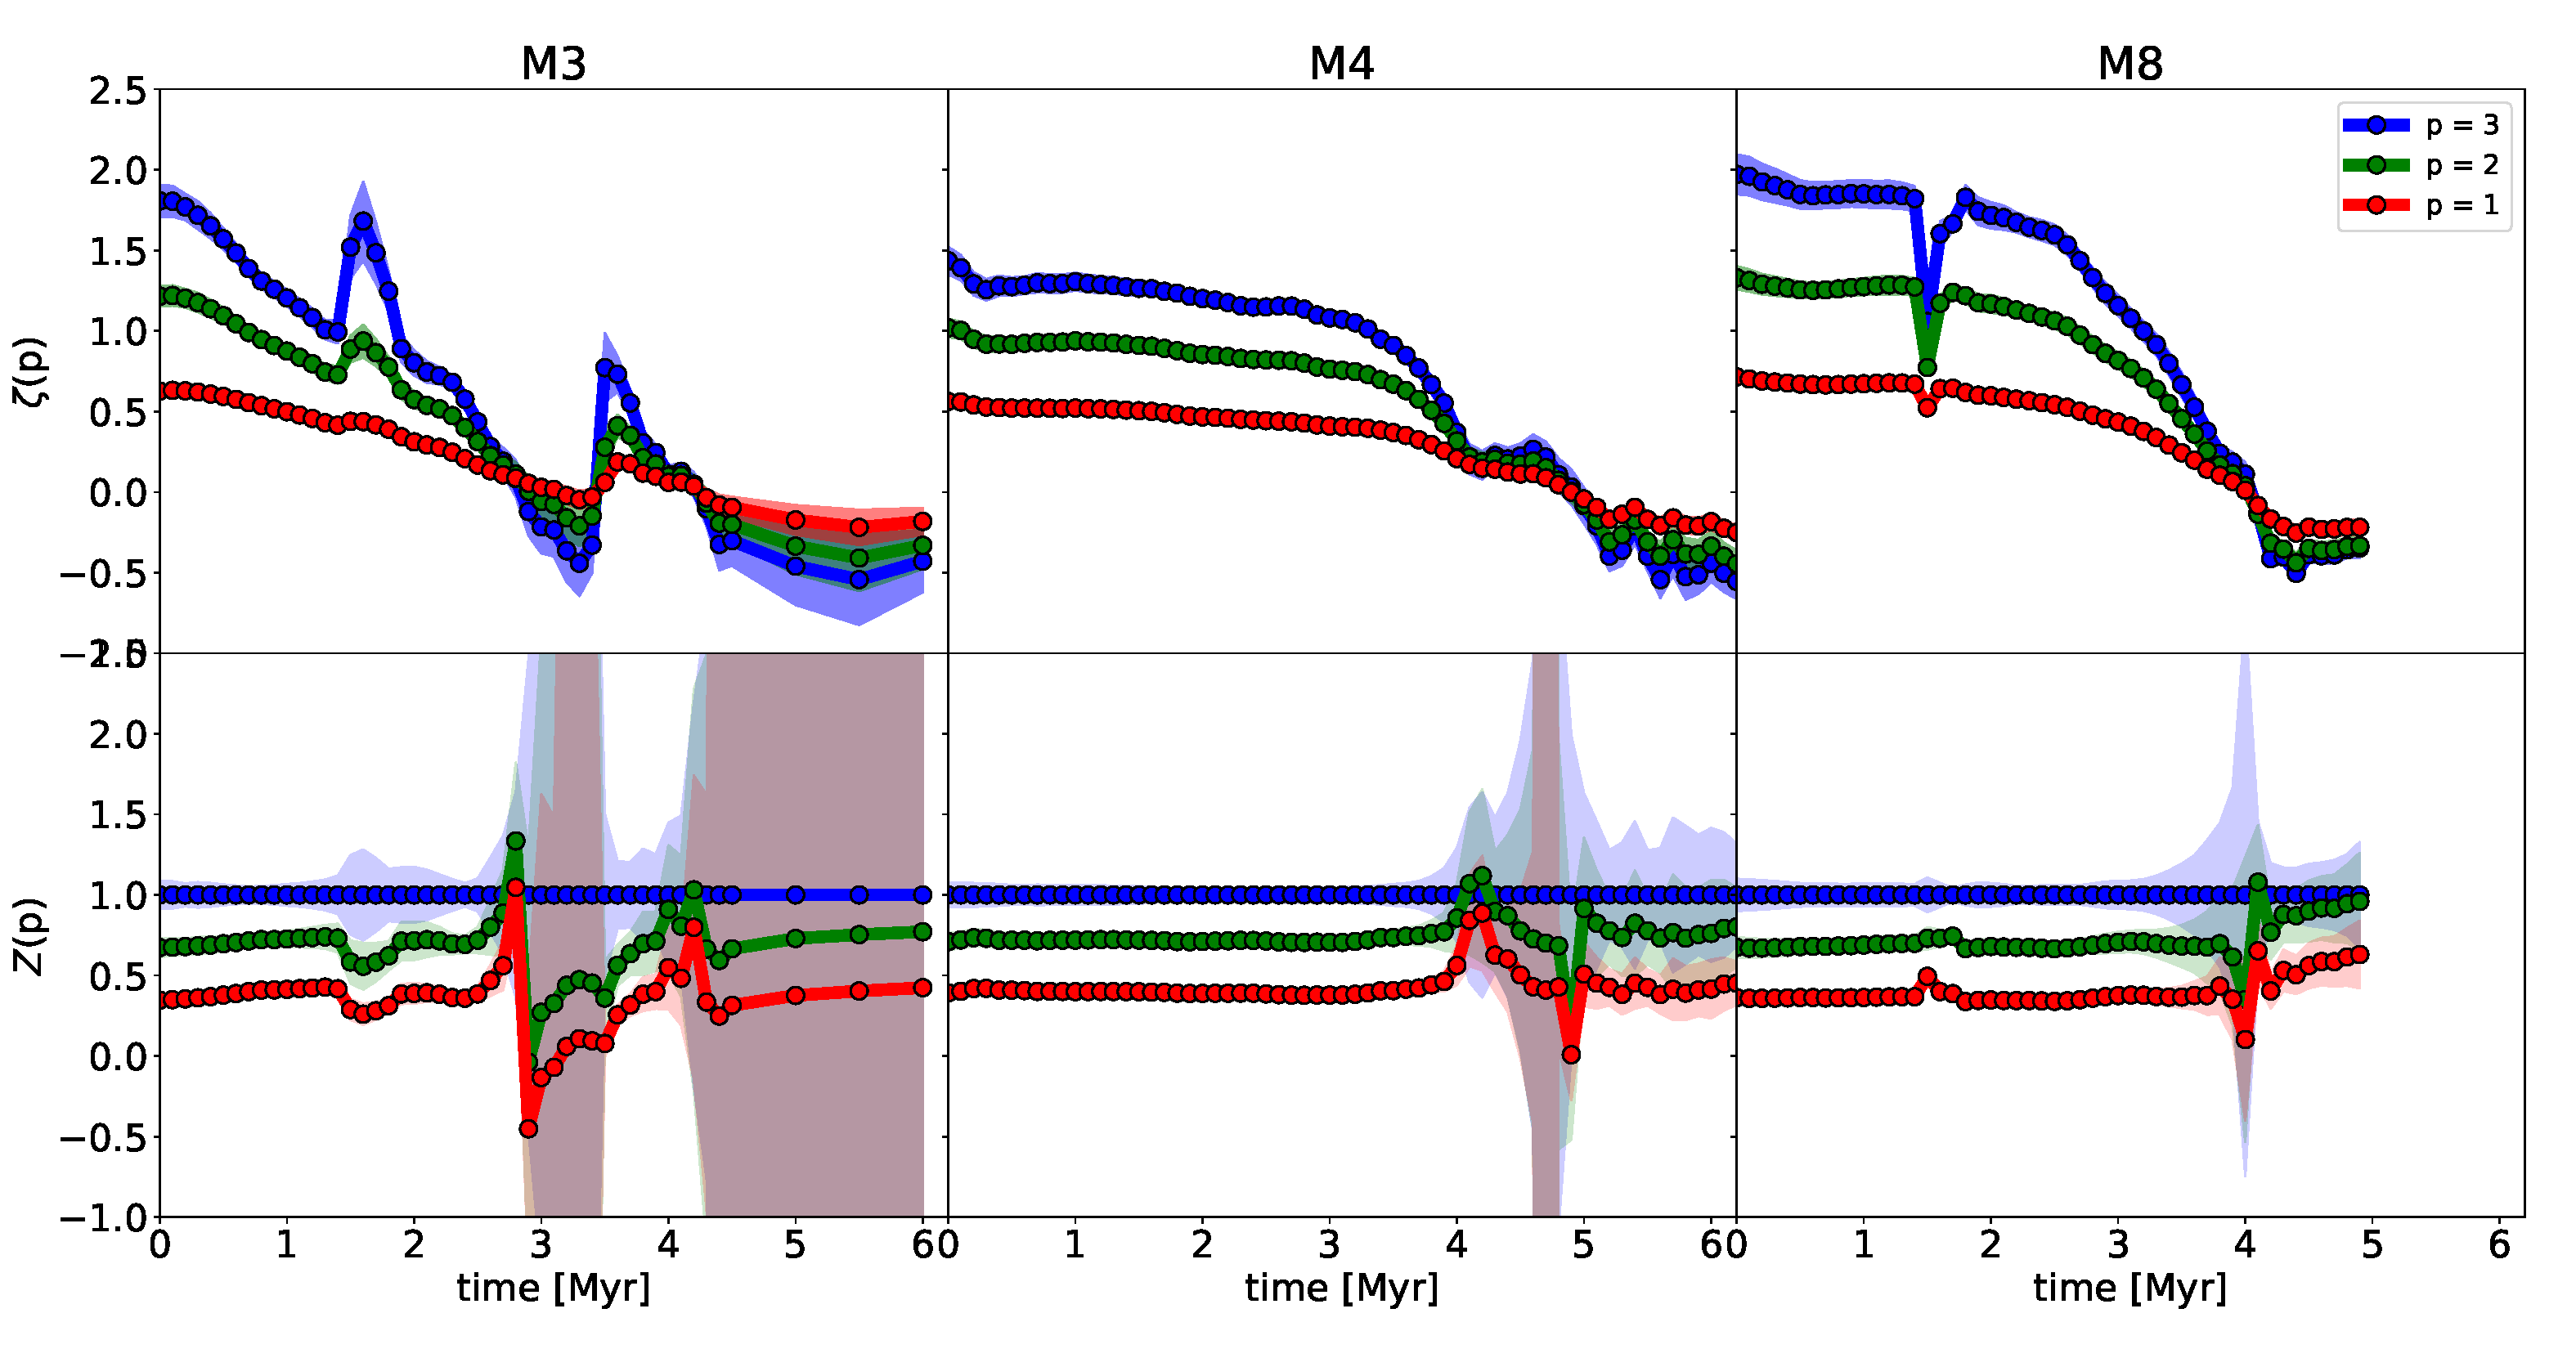
\includegraphics[width=\textwidth]{error_vsf04_zeta_z.pdf}
    \caption{
        Like Fig.~\ref{pic:results:zeta_all}a.
        Additionally, the shaded areas behind the data represent the error ranges of computed $\zeta$ (\textit{top}) and $Z$ (\textit{bottom}), respectively. 
    }
    \label{pic:appFitting:error_vsfhr04_zeta_z}
\end{figure*}

\textbf{
    From \texttt{curve_fit} we also obtain the $\chi^2$ errors for measured $\zeta$. 
    In Fig.~\ref{pic:appFitting:error_vsfhr04_zeta_z} we show a reduced version of Fig.~\ref{pic:results:zeta_all}(a).
    This means that we only plot the time evolution of $\zeta$ for all three clouds.
    Additionally, we added shades of the same colours of the respective lines that represent the error areas as derived by \texttt{curve_fit}.
    We see that as long as the VSFs are not too flat in the inner and intermediate regions, meaning that $|\zeta|\,\gtrsim$~\rc{!!! 0.1 !!!} the relative errors $\Delta \zeta / \zeta$ are within a range of 5--12\%. 
    If the VSFs are, however, flat the level of relative errors increases to several as even small changes in $\zeta$ can have significant impact. 
}

\rc{continue}




\endinput
